\section{Validating proof trees}

After introducing the problem and modelling in Lean, we now describe the algorithm to verify a solution. In this chapter we deal with the soundness, which means here that every atom in the interpretation is actually in the semantics. For this we use the proof trees as the certificate and the proof theoretic semantics.

A ground atom is in the proof theoretic semantics if there exists a valid proof tree, that has this ground atom as its head. We were provided with all the proof trees and checking the heads is rather easy, so what remains to be checked is the validness of a proof tree, that was defined in the previous chapter.

\begin{lstlisting}
    def isValid(P: program τ) (d: database τ) (t: proofTree τ): 
    Prop :=
    match t with
    | proofTree.node a l => 
    ( ∃(r: rule τ) (g:grounding τ), 
        r ∈ P ∧ 
        ruleGrounding r g = groundRuleFromAtoms a (List.map root l)
        ∧ l.attach.All₂ (fun ⟨x, _h⟩ => isValid P d x)) 
    ∨ (l = [] ∧ d.contains a)
\end{lstlisting}

The second part of this disjunction consists of a database check and an easy check of list emptyness. The first part is more interesting. Since we use there existential quantifiers, we have to implement something to check this. As the program is given as a list of rules, we can simply iterate over this list. For the grounding we however can something more sophisticated, but groundings are not our object of choice for that.


\subsection{Substitutions}
    A grounding is function from variables to constants. This mean that we always need to specify for every variable a constant that it is mapped to. This was good in the definitions to ensure that we always get a ground atom, but raises in the unification case problems as the following example demonstrates.

    \begin{example}
        Consider the signature consisting of $C = \{a,b,c\}$, $V = \{x,y,z \}$ and $R = \{R\}$. Suppose we want to match a list of terms with a list of constant. The first term is $t_1 = x$ and the first constant is $a$. We might use the the grounding $g = x \mapsto a, y \mapsto a, z \mapsto a$.

        Now we want to use this result and match another term $t_2 = y$ with the constant $b$. The variable $y$ is already mapped to a different constant, but we cannot say whether this is due to a previous matching process or simply because we needed to define a value for every input.
        

        
    \end{example}

    Instead, we want to use substitutions that were already introduced in \cite{datalogCoq}. A substitution is a partial mapping from variables to constants. We implement this by mapping to an Option of constant.

    \begin{lstlisting}
    def substitution (τ: signature):= τ.vars → Option (τ.constants)
    \end{lstlisting}

    This allows us to only specify what is necessary. If we apply a substitution to a term, we only replace a variable by a constant, if the substitution is defined for this variable and the constant will be the result of the substitution in this case.

    \begin{lstlisting}
    def applySubstitutionTerm (s: substitution τ) (t: term τ): term τ :=
    match t with
    | term.constant c => term.constant c
    | term.variableDL v => 
        if p: Option.isSome (s v) 
        then term.constant (Option.get (s v) p) 
        else term.variableDL v
    \end{lstlisting}

    We can use similar defintions as previously for groundings to apply substitutions to atoms or rules.

    The main result we want to prove is the following.

    \begin{lstlisting}
    theorem groundingSubstitutionEquivalence 
        [Nonempty τ.constants] (r: groundRule τ) (r': rule τ):
        (∃ (g: grounding τ), ruleGrounding r' g = r) ↔ 
        (∃ (s: substitution τ), applySubstitutionRule s r'= r)
    \end{lstlisting}

    This allows us to replace the grounding check by a substitution check, when trying to validate trees and by this we can bypass the problems that were illustrated in the example above. 

    For the forward implication, we can transform any grounding in a simple way to a substitution. In this substitution every value is defined with the value of the grounding.

    \begin{lstlisting}
    def groundingToSubstitution (g: grounding τ): substitution τ
        := fun x => Option.some (g x)
    \end{lstlisting}

    It is very easy to prove that this is equivalent on every rule.

    For the back direction, we need additionally that the set of constants is non-empty. We can ensure this during the input phase by adding a fresh constant symbol to the constant symbols similar to Herbrand universes. This symbol does not appear in any proof trees and does not influence the results. Since we only look at safe programs, it will also not introduce any new ground atoms to the model.

    The following example shows the problems that occur without the non-emptyness assured.

    \begin{example}
        Consider the program $P= \{p \leftarrow, q \leftarrow p\}$ and the signature $C = \emptyset$, $V = \{x,y,z \}$ and $R = \{p,q\}$

        Any rule in $P$ is already a ground rule and there exists a substitution, the empty substitution that maps all variables to none, so that the rule is equal to itself as a ground rule.
        
        There is however no grounding that can achieve this. We cannot define a grounding since we have no constant available, but have variables that need to be mapped somewhere. Therefore the equivalence does not hold here.
    \end{example}

    Since the set of constants is non-empty, we can use the axiom of choice to get values for which the substitution is not defined.

    \begin{lstlisting}
    noncomputable def substitutionToGrounding 
        [ex: Nonempty τ.constants] (s: substitution τ): grounding τ := 
        fun x =>    if p:Option.isSome (s x) 
                then Option.get (s x) p 
                else Classical.choice ex

    \end{lstlisting}

    When introducing substitutions, we had the goal to only add what is needed to a substitution and usually we want the smallest possible substitution. In order to formalize this, we want to define a linear relation on substitutions, that is denoted by $\subseteq$

    Firstly, we define the substitution domain of a substitution as the set of variables for which the substitution is defined. 

    \begin{lstlisting}
    def substitution_domain (s: substitution τ): Set (τ.vars) := 
        {v | Option.isSome (s v) = true}
    \end{lstlisting}

    A substitution $s_1$ is then a subset of a substitution $s_2$, if both substitutions agree on the substitution domain of $s_1$. Outside of this $s_1$ is never defined, whereas $s_2$ might be, so that we view $s_1$ as smaller.

    \begin{lstlisting}
    def substitution_subs (s1 s2: substitution τ): Prop :=
    ∀ (v: τ.vars), v ∈ substitution_domain s1 → s1 v = s2 v
    \end{lstlisting}

    This can be proven to be a partial order.

\subsection{Unification}

We know that instead of finding a grounding, it suffices to find a substitution. Now we want to describe an algorithm that tells us whether the ground rule that is formed from a node of the proof tree is the substituted rule of some rule of the program. For this we take inspiration from the unification problem of first-order logic.

In the unification problem we are given a set of equations between first-order terms and are required to present the most-general unifier.

Our problem is similar. The equations will not be between terms, but between an object and a ground object of the same corrosponding type and we require a substitution that solves all equations and is minimal in our subset relation.

An algorithm to solve the first-order unfication problem is the algorithm of Martelli and Montanari \cite{MartMont} and is depicted below:
\begin{algorithm}
    \caption{Algorithm of Martelli and Montanari}
\begin{algorithmic}
    \While {There exists some equation for which a transformation is possible}
    \State Pick this equation $e$ and do one of the following steps if applicable
    \begin{enumerate}
        \item If $e$ is of the form $t = t$, then delete this equation from the set.
        \item If $e$ is of the form $f(t_1, .., t_n) = f(s_1,.., s_n)$, then delete $e$ and add $n$ new equations of the form $t_i = s_i$
        \item If $e$ is of the form $f(t_1, .., t_n) = g(s_1,.., s_m)$ with $g \neq f$, then stop and reject.
        \item If $e$ is of the form $f(t_1,..,t_n) = x$ for a variable $x$ and delete $e$ and add an equation with the swapped order to the set
        \item If $e$ is of the form $x=t$ for some variable $x$, then check if x occurs in t. If it does, then stop and reject. If not map all $x$ to $t$ in the set.
    \end{enumerate}
    \EndWhile
\end{algorithmic}
\end{algorithm}

This algorithm offers a good starting point for our own algorithm, but we certain transformation can't occur in the limited syntactic form we operate in. Additionally, we want to output a substitution instead of just answering whether a substitution exists. It is sufficient to do it here, but will later be important. Instead of mapping all $x$ to $t$ as done there in step 5, we will add $x\mapsto t$ to a substitution that is presented as an input. If a variable occurs on the left side, we will check whether it is already in the domain of the substitution and if so check if its current value is consistent with the right side.
As function symbols appart from constant symbols are not allowed, we can simplify steps 2 and 3, as we never add new equations and instead only check if the constant symbol matches. Finally, as the one side of the equation is always a ground object there will never be a variable on this side, so that we do not have to swap the equation as in step 4.

We will start with matching a term to a constant with the following algorithm.

\begin{lstlisting}
    def matchTerm (t: term τ)(c: τ.constants) (s: substitution τ):
    Option (substitution τ) :=
    match t with
    | term.constant c' =>
        if c = c'
        then Option.some s
        else Option.none
    | term.variableDL v =>
        if p:Option.isSome (s v)
        then  if Option.get (s v) p = c
            then
                Option.some s
            else
                Option.none
        else extend s v c
\end{lstlisting}

We are given a term $t$, a constant $c$ and a current substitution $s$ and want to return the minimal substitution $s'$ so that $s \subseteq s'$ and applying $s'$ to $t$ will make it equal to $c$ or none if no such $s'$ exists.

This is done by case distinction. If $t$ is a constant, then we either return $s$ if $t$ is equal to $c$, or return none as two different constants can not be unified by a substitution. If $t$ is variable, we check if $t$ is in the domain of $s$. If it is already defined we check if the value matches the required value. If it is not defined we extend $s$ with the new mapping $v \mapsto c$.
Formally extend is defined in the following way:

\begin{lstlisting}
    def extend (s: substitution τ) (v: τ.vars) (c: τ.constants) :
        substitution τ 
    := fun x => if x = v then Option.some c else s x
\end{lstlisting}

We know formally prove the correctness of this algorithm. The first result is that if \texttt{matchTerm} returns a substitution $s'$ that $s'$ is indeed a solution, i.e. that applying $s'$ to $t$ results in $c$ and that $s'$ is an extension of $s$

\begin{lstlisting}
    lemma matchTermFindsSolution (t: term τ) (c: τ.constants) 
    (s: substitution τ) (h: Option.isSome (matchTerm t c s)): 

    applySubstitutionTerm (Option.get (matchTerm t c s) h) t = c 
    ∧ s ⊆ (Option.get (matchTerm t c s) h)
\end{lstlisting}
\begin{proof}
The proof is done via case distinction. Suppose firstly that $t$ is a constant $c'$. Since matchTerm returned a substitution we must have that $c$ and $c'$ are the same constant and therefore $s'$ is $s$. Applying a substitution to a constant does not change it, so $s' t = s' (c') = c' = c$. Additionally since $\subseteq$ is a linear order and $s' = s$, we have that $s \subseteq s'$

Now we assume that $t$ is a variable $v$. Now we do another case distinction on whether $s v$ is defined or not. If it is defined, $v$ must already be mapped to $c$ and we return $s$ as this is a solution as seen previously. If it would be mapped to something else, then matchTerm would return none, which would be in violation to our assumptions.
If it is not defined, we use extend. After that $v$ is mapped to $c$, so that $s' t$ will be equal to $c$. Now we finally have to show that $s \subseteq$ extend $s$ $v$ $c$. We only change the value of $v$. Since $v$ was not defined earlier, for any variable in the domain of $s$, $s$ and extend $s$ $v$ $c$, so that it is fulfilled.
\end{proof}

We have proven so far the matchTerm returns a solution, but it might not be a minimal solution. When we want to match atoms with ground atoms, we need to match a list of terms with a list of constants. There it is important that the returned substitution is indeed minimal to conclude whether a solution exists as the following example shows.

\begin{example}
    Consider the list of terms $l_1 = [x, y, x]$ with the variables $x$ and $y$ and the list of constants $l_2 = [a,b, c]$. We want to find a substitution that we can apply to $l_1$ to gain $l_2$ if possible. We start with the empty substitution and first want to match the first elements of $l_1$ and $l_2$. If we receive a solution $s$, then we continue with the next elements of $l_1$ and $l_2$, but this time the matching extends $s$ instead of the empty substitution.

    Now suppose the procedure $P_1(t,c, s)$ that takes a term, a constant and a substitution does not always return a minimal solution. So it might return for $x$, $a$ and the empty substitution the substitution $s = x \mapsto a, y\mapsto a$.

    Now we again call $P_1$ with $y$, $b$ and $s$. $P_1$ will not return anything, because $y$ is already mapped to something else. From this fact we cannot conclude that there exists no solution at all however. In fact, the non-minimality of the results of $P_1$ prevents this reasoning.

    If we have a second procedure $P_2(t,c, s)$ that always returns the minimal solution we solve the matching process for the first two list elements of each list to return $s' = x \mapsto a, y \mapsto y$. Now we want to match $x$ with $c$ and $P_2$ will return none. We can conclude that no solution exists since any substitution from $P_2$ is minimal. If there exists a solution to the list then $l_2$, it necessarily must match the first to elements of both lists. Since $s'$ is the minimal solution of a process that started with the empty substitution and always returned minimal solution, any solution to the list must extend $s'$. Therefore it must agree on the domain of $s'$ and therefore it must map $x$ to $a$ and therefore no solution can exist.

\end{example}

\begin{lstlisting}
    lemma matchTermFindsMinimalSolution' (t: term τ) 
    (c: τ.constants) (s: substitution τ) 
    (h: Option.isSome (matchTerm t c s)): 
    
    ∀ (s': substitution τ),(s ⊆ s' ∧ applySubstitutionTerm s' t = c)
        → (Option.get (matchTerm t c s) h) ⊆ s' :=
\end{lstlisting}
\begin{proof}
This is again done via case distinction on the type of $t$. If $t$ is constant, then $s'$ must be equal to $s$. For any $s^\ast$ with $s \subseteq s^\ast \land s^\ast t = c$ we have b that $s' \subseteq s^\ast$ by the assumption of the property of $s^\ast$

Now we consider the case of $t$ being a variable $v$ and do a case distinction whether $s v$ is defined. If it was already defined, then $s'$ must again be equal to $s$, so that the claim is fulfilled by the argument above.
If $s v$ was not defined, we have to show that extend $s$ $v$ $c$ is a subset of any such $s^\ast$. We assume for a contradiction that this is not the case. Then there must be a variable in the domain of extend $s$ $v$ $c$ such that extend $s$ $v$ $c$ and $s^\ast$ differ. Suppose this variable is $v$. Then $s^\ast$ would either not be defined for $v$ or map $v$ to some other constant $c'$. In both cases $s^\ast v \neq c$, so that $s^\ast$ would not be a solution and we would have reached a contradiction.
If it is some other variable $v'$, then the value of extend $s$ $v$ $c$ is simply the value of $s$. Since $s^\ast$ maps $v$ to a different value compared $s$, $s$ would not be a subset of $s^\ast$ and we have reached another contradiction.
\end{proof}

So we know that if matchTerm returns a substitution then it is a minimal solution. We additionally have to prove that if matchTerm does not return a substitution that then no solution exists.

\begin{lstlisting}
    lemma matchTermNoneImpNoSolution (t: term τ)
        (c: τ.constants) (s: substitution τ)
        (h: Option.isNone (matchTerm t c s)):
    
    ¬ (∃(s': substitution τ), s ⊆ s'∧applySubstitutionTerm s' t = c)
\end{lstlisting}
\begin{proof}
This is again done via case distinction on the type of $t$. If $t$ is a constant $c'$, then $c'$ must be different from $c$, so that matchTerm returns none. Then no substitution can map $t$ to c.

If $t$ is a variable $v$, then $s v$ must be defined and mapped to a different value compared to $c$. Then again no such $s'$ can exist. If $s$ would be a subset of $s'$, then $s'$ would not unify $t$ with $c$ and if $s'$ would unify $t$ with $c$ then $s$ would not be a subset of $s'$.
\end{proof}

After proving the correctness for terms we now want to move up to atoms. Unfortunately, we cannot use recursion directly on the term list of an atom. An atom requires a proof that the length of the list is equal to the arity of the relation symbol, which fails when we do recursion on the list. Therefore we first establish a new procedure that matches a list of terms with a list of constants, if possible.

\begin{lstlisting}
    def matchTermList (s: substitution τ) (l1: List (term τ))
        (l2: List (τ.constants)): Option (substitution τ) :=
    match l1 with
    | List.nil => some s
    | List.cons hd tl =>
        match l2 with
        | List.nil => none
        | List.cons hd' tl' =>
        let s' := matchTerm hd hd' s
        if p: Option.isSome s'
        then matchTermList (Option.get s' p) tl tl'
        else none
\end{lstlisting}

Here we are given as previously a substitution as an input with the two lists. For the correctness it is required that both lists have the same length, but this is the case for atoms. If the first list is empty we return the substitution. If instead it has a first element and the second list has as well a first element, we match these elements using matchTerm and if this results in a solution, we return the result of matchTermList with the remaining lists and the resulting substitution.

As previously, we have to prove the correctness of this algorithm. We again want to show that the algorithm returns the minimal solution iff it exists. We require for these results that both lists are the same length. If the list of constants is longer than the list of terms, the \texttt{matchTermList} function may return a solution eventhough the lists will never be equal. As we only want to use this to match atoms, this is however not a problem. No subsititution can change the symbol, so that we will only try to match atoms with ground atoms that have the same symbol. The symbol determines the number of terms so that both lists will have the same length.

\begin{lstlisting}
    lemma matchTermListFindsSolution (s: substitution τ)
    (l1: List (term τ)) (l2: List (τ.constants))
    (len: l1.length = l2.length)
    (h:Option.isSome (matchTermList s l1 l2)):
        List.map (applySubstitutionTerm (Option.get (matchTermList s l1 l2) h)) l1 
        = List.map term.constant l2 
        ∧ s ⊆ (Option.get (matchTermList s l1 l2) h ) :=
\end{lstlisting}
\begin{proof}
    We prove this by induction on $l_1$ for arbitrary $s$ and $l_2$.
    In the base case $l_1$ is the empty list. Since both lists have the same length $l_2$ must also be the empty list. matchTermList then returns $s$. Applying this to an empty list returns an empty list. Therefore the base case is complete.

    In the induction step we have that $l_1$ is of the form $hd::tl$ and we can similarly assume that $l_2$ is of the form $hd'::tl'$ and that $tl$ and $tl'$ have the same length by our assumption. Since matchTermList returned a substitution, matchTerm $hd$ $hd'$ also must return a substitution $s^\ast$.
    We then use this as an input to gain $s'$ from matchTermList $s^\ast$ $tl$ $tl'$. By the induction hypothesis $s^\ast \subseteq s'$ and applying $s'$ to $tl$ results in it being equal to $tl'$. To show that both lists are equal, we just have to show that after applying $s'$ the heads will be equal. We know that applying $s^\ast$ to $hd$ will result in it being equal to $hd'$. Since $s^\ast \subseteq s'$ and our previous result that if a substitution maps a term to a constant then extension of this substitution will also map the term to the same constant, we have this.
    Lastly, we have to show that $s \subseteq s'$. From the correctness proof of matchTerm we know that $s \subseteq s^\ast$ and from the induction hypothesis we know that $s^\ast \subseteq s'$. Since $\subseteq$ is transitive, the result follows.
\end{proof}

After proving that it is a solution, we prove that the solution is minimal.

\begin{lstlisting}
    lemma matchTermListFindsMinimalSolution (s: substitution τ)
    (l1: List (term τ)) (l2: List (τ.constants)) 
    (len: l1.length = l2.length) 
    (h: Option.isSome (matchTermList s l1 l2)):
    ∀ (s': substitution τ), 
        List.map (applySubstitutionTerm s') l1 = List.map term.constant l2
        ∧ s ⊆ s' → (Option.get (matchTermList s l1 l2) h ) ⊆ s' :=
\end{lstlisting}
\begin{proof}
    We prove this again via induction on $l_1$ for arbitrary $l_2$ and $s$. If $l_1$ is empty, we return $s$ and the claim is true by assumption.

    In the induction step we have that $l_1$ has the form $hd::tl$ and we can assume that $l_2$ has the form $hd'::tl'$ and that $tl$ and $tl'$ have the same length. Additionally, we know that matchTerm $hd$ $hd'$ s returns a substitution $s^\ast$. From the induction hypothesis we know that matchTermList $s^\ast$ tl tl' $\subseteq \hat{s}$ for any substitution $\hat{s}$ that extends $a^\ast$ and maps $tl$ to $tl'$. Since $s^\ast$ is a minimal solution for $hd$ and $hd'$ and $s^\ast$ only extends it, we know that it is a solution for the whole list. We also know from the minimality of $s^\ast$ that $s \subseteq s^\ast$. From the induction hypothesis, we get that $s^\ast \subseteq \hat{s}$. Transitivity tells us that $s \subseteq \hat{s}$ as 
\end{proof}

Finally the negative case that confirms that the return value of none does indeed state that there is no solution.

\begin{lstlisting}
    lemma matchTermListNoneImplNoSolution (s: substitution τ)
    (l1: List (term τ)) (l2: List (τ.constants))
    (len: l1.length = l2.length) 
    (h: Option.isNone (matchTermList s l1 l2)): 
    ∀ (s': substitution τ), s ⊆ s' →
    ¬  List.map (applySubstitutionTerm s') l1 = List.map term.constant l2 :=
\end{lstlisting}
\begin{proof}
    We prove this again via induction on $l_1$ for arbitrary $l_2$ and $s$. If $l_1$ is the empty list, we cannot return none. As the prerequisite is not fulfilled, the statement is correct.

    In the induction step we have that $l_1$ has the form $hd::tl$ and we can assume that $l_2$ has the form $hd'::tl'$ and that $tl$ and $tl'$ have the same length. There are two cases where matchTermList can return none. The first case is when matchTerm $hd$ $hd'$ $s$ returns none. If that is the case there is no $s'$ with $s\subseteq s'$ and applying $s$ to $hd$ will make it equal to $hd'$. Therefore the two lists cannot be equal either and the proof is finished.

    If matchTerm $hd$ $hd'$ $s$ returns a substitution $s^\ast$, then matchTermList $s^\ast$ $tl$ $tl'$ must return none. From the induction hypothesis we know that there is no substitution $s'$ with $s^\ast \subseteq s'$ and applying $s'$ to $tl$ bringing it equal to $tl'$. Since $s^\ast$ is already the minimal solution to match $hd$ with $hd'$ there cannot exist a solution here.
\end{proof}

This can be used to create a matchAtom procedure. We are given an atom and a ground atom and check if the symbols are equal. If they are, we also get that their term lists must be equal as the length of the term list is equal to the arity of the relation symbol. The same symbol implies the same length.
If the symbols are different, we will never unify them.

\begin{lstlisting}
    def matchAtom (s: substitution τ) (a: atom τ) (ga: groundAtom τ):
    Option (substitution τ) :=
        if a.symbol = ga.symbol
        then
            matchTermList s a.atom_terms ga.atom_terms
        else none
\end{lstlisting}

The correctness proofs follow from the proofs of matchTermList since we already established the same length of both lists from the symbol.

Now we can create a \texttt{matchAtomList} function similarly to \texttt{matchTermList} and use this to define a \texttt{matchRule} function. We first try match the head of the rule with the head of the ground rule. If this returns a solution, we use this as the start for matching the bodies. If not, we will not find a solution and return none.

\begin{lstlisting}
    def matchRule (r: rule τ) (gr: groundRule τ):
        Option (substitution τ):=
        let s := matchAtom emptySubstitution r.head gr.head
        if p: Option.isSome s
        then matchAtomList (Option.get s p) r.body gr.body
        else none

\end{lstlisting}

We know prove again that if this returns a substitution then this is a solution and if none is return then there is no solution using our previous results. For both these results we assume that both bodies have the same length, but determining the length of a list can be done in the tree validation process.
We want a statement with the quantifier to combine it with the theorem about the equivalence between groundings and substitutions. We can prove this statement by using the result of \texttt{matchRule} as a witness for the quantifier. For the back direction, we see that this statement implies that a solution exists, which we always find with \texttt{matchRule}

\begin{lstlisting}
    theorem matchRuleIsSomeIffSolution (r: rule τ) (gr: groundRule τ) 
    (len: r.body.length = gr.body.length): 
    Option.isSome (matchRule r gr) ↔ 
    ∃ (s: substitution τ), applySubstitutionRule s r = gr
\end{lstlisting}

We now have a method to replace this quantifier by a computable function and can finally devise the check for tree validation.

\subsection{Tree validation}

We have so far introduced introduced substitutions and have shown a way to decide whether a substitution exists that maps a rule to a ground rule. Now we want to finally show a way to validate trees. As the first step we want to find whether a ground rule $gr$ we gain from the tree is in the ground program, i.e. that there exists a grounding $g$ (or from the previous results a substitution $s$) and a rule $r$ from the program $P$, so that applying $g$ to $r$ yields $gr$. We want to use the \texttt{matchRule} function defined earlier for this. This function required that both bodies of the rules to have the same length in order to work properly. Instead of just computing the length we want to do a bit more. We previously noted that substitutions (or groundings) never change the symbol of an atom, so that we do not have to try to match rules whose symbols differ. The symbols of a rule are expressed in the symbol sequence.

\begin{lstlisting}
    def symbolSequence (r: rule τ): List τ.relationSymbols := 
        r.head.symbol::(List.map atom.symbol r.body)

\end{lstlisting}

We can now compare the symbol sequence of a rule and the symbol sequence of a ground rule. If they are equal, we see that the bodies have the same length, since we just map each body element and attached for both the head at the front. If they are however not equal, then no substitution can be applied to the rule so that it will yield the ground rule.

We can use this to check whether a ground rule $gr$ is in the ground program of $P$ by computing the symbol sequence of $gr$ and comparing it with the symbol sequence of every rule in the program. For those rules where the symbol sequences are equal, we can apply the \texttt{matchRule} function until we find the first matching rule. While this work, we have to iterate in the worst case always over the whole program. Instead we can preprocess the program into a function that returns for a symbol sequence a list of rules with the same symbol sequence.

\begin{lstlisting}
    def parseProgramToSymbolSequenceMap (P: List (rule τ)) 
    (m: List τ.relationSymbols → List (rule τ)): 
    List τ.relationSymbols → List (rule τ) :=
    match P with
    | [] => m
    | hd::tl =>
        let seq:= symbolSequence hd
        parseProgramToSymbolSequenceMap tl 
            (fun x => if x = seq then hd::(m x) else m x)
\end{lstlisting}

By induction we can prove that any symbol sequence $s$ the result of 

\texttt{parseProgramToSymbolSequenceMap P m} returns a the list consisting of those rules in $P$ whose symbol sequence matches $s$ and those rules that in $m (s)$. If we therefore use a function that maps any symbol sequence to the empty list for m we get exactly the list of rules that match a particular symbol sequence. As only those rules can result into the ground rule $gr$ with the symbol sequence $s$ by applying a grounding $g$, its enough to iterate over those rules. The \texttt{List.any} function does this and returns true as soon \texttt{matchRule} returns a \texttt{some}. The preprocesssing of $P$ is given as a function $m$, so that it only will be done once.  

\begin{lstlisting}
    def checkRuleMatch (m: List τ.relationSymbols → List (rule τ)) 
    (gr: groundRule τ) (ruleToString: rule τ → String)
    : Except String Unit :=
    if List.any (m (symbolSequence gr.toRule)) 
        (fun x => Option.isSome (matchRule x gr)) = true
    then Except.ok ()
    else Except.error ("No match for " ++ ruleToString gr)
\end{lstlisting}

If $m$ is the result of \texttt{parseProgramToSymbolSequenceMap} of $P$ and a function that maps anything to the empty list, \texttt{checkRuleMatch} returns ok if and only if there is a rule $r$ in $P$ and a grounding $g$ such that applying $g$ to $r$ results in the ground rule $gr$.

\begin{lstlisting}
    lemma checkRuleMatchOkIffExistsRuleForGroundRule 
    (m: List τ.relationSymbols → List (rule τ)) (P: List (rule τ)) 
    (gr: groundRule τ) (ruleToString: rule τ → String ) 
    (ssm: m = parseProgramToSymbolSequenceMap P (fun _ => [])): 
    checkRuleMatch m gr ruleToString = Except.ok () 
    ↔ ∃ (r: rule τ) (g:grounding τ),r ∈ P ∧ ruleGrounding r g = gr
\end{lstlisting}

In order to start validating we need another helper function. The tree validation function will return an element of type \texttt{Except String Unit}, so that if the tree is invalid an Exception with an error message in a String is thrown. If it is valid, then nothing is return. In order to show that a tree with the root $a$ is valid, we have to show that all direct subtrees of $a$ are valid using the same function. We could use \texttt{List.all (Except.isOk)} and this would return true iff all subtrees are valid. We would however loose the error message. Instead we define the following function, that returns the first error message it finds.

\begin{lstlisting}
    def List.map_except_unit {A B: Type} (l: List A) 
    (f: A → Except B Unit): Except B Unit :=
    match l with
    | [] => Except.ok ()
    | hd::tl =>
        match f hd with
        | Except.ok () => List.map_except_unit tl f
        | Except.error b => Except.error b
\end{lstlisting}

By induction we prove that it returns \texttt{ok ()} iff for all elements in the list $f$ is evaluated to \texttt{ok ()}.

\begin{lstlisting}
    lemma List.map_except_unitIsUnitIffAll {A B: Type} (l: List A) 
    (f: A → Except B Unit): 
    List.map_except_unit l f = Except.ok () 
    ↔ ∀ (a:A), a ∈ l → f a = Except.ok ()
\end{lstlisting}

In order to validate a tree we have to consider two cases. If it has no children, then it is a fact. This fact may be part of the database or it may be a fact in the program. We can detect if the list of children is empty and ask the database whether it contains the root. If that is the case, the tree is valid and we return \texttt{ok ()}. If not, we use \texttt{checkRuleMatch} to find a fact for the root in $P$ and return the result. Since the tree has no children, all children are valid as well.
If it has children we try to find a rule using \texttt{checkRuleMatch} that matches the current node and its children and if that is the case we check that all children are valid using the \texttt{List.map\_except\_unit} function.

\begin{lstlisting}
    def treeValidator (m: List τ.relationSymbols → List (rule τ)) 
    (d: database τ)(t: proofTree τ) (ruleToString: rule τ → String):
        Except String Unit :=
    match t with
    | tree.node a l =>
        if l.isEmpty
        then    if d.contains a
                then Except.ok ()
                else
                    match checkRuleMatch m 
                    {head:= a, body := []} ruleToString with
                    | Except.ok _ => Except.ok ()
                    | Except.error msg => Except.error msg
        else
            match checkRuleMatch m 
            {head:= a, body := List.map root l} ruleToString with
            | Except.ok _ => 
                List.all l.attach (fun ⟨x, _h⟩ => Except.isOK 
                (treeValidator m d x ruleToString))
            | Except.error msg => Except.error msg
\end{lstlisting}

By induction on the height of the tree we can prove the correctness of this algorithm as the children have a smaller height than the tree.

\begin{lstlisting}
    lemma treeValidatorOkIffIsValid 
    (m: List τ.relationSymbols → List (rule τ)) 
    (P: List (rule τ)) (d: database τ) (t: proofTree τ) 
    (ruleToString: rule τ → String) 
    (ssm: m = parseProgramToSymbolSequenceMap P (fun _ => [])): 
    
    treeValidator m d t ruleToString = Except.ok () 
    ↔ isValid (List.toFinset P) d t :=

\end{lstlisting}

As we want to validate the whole result of a datalog program, we will often need many proof trees and a function that can validate them. Additionally, we need to preprocess the program to gain the map from symbol sequences to rules. This is done in the following function.

\begin{lstlisting}
    def validateTreeList (P: List (rule τ)) (d: database τ) 
    (l: List (proofTree τ)) 
    (ruleToString: rule τ → String): Except String Unit :=
    let m:= parseProgramToSymbolSequenceMap P (fun _ => [])
    List.map_except_unit l 
        (fun t => treeValidator m d t  ruleToString)

\end{lstlisting}

Using the properties of \texttt{treeValidator} and \texttt{List.map\_except\_unit}, we can show that this function returns \texttt{ok ()} iff all trees in \texttt{l} are valid. We know that a ground atom $ga$ is in the \texttt{proofTheoreticSemantics} if there exists a proof tree with the root $ga$, so that we can conclude the set of roots of the trees in $l$ is a subset of the semantics. In order to get an iff statement, we also have to include that all trees are valid, because a root preserving permutation of a proof tree will in general not be valid and therefore \texttt{validateTreeList} will report an error, but its root is still in the semantics.

\begin{lstlisting}
    lemma validateTreeListUnitIffSubsetSemanticsAndAllElementsHaveValidTrees 
    (P: List (rule τ)) (d: database τ) (l: List (proofTree τ)) 
    (ruleToString: rule τ → String) : 
    validateTreeList P d l  ruleToString = Except.ok () ↔ 
        {ga: groundAtom τ| ∃ (t: proofTree τ), t ∈ l ∧ root t = ga } ⊆ proofTheoreticSemantics P.toFinset d 
        ∧ ∀ (t: proofTree τ), t ∈ l → isValid P.toFinset d t
\end{lstlisting}

It turns out however that we can do a bit better and prove a stronger statement as the following example shows.
\begin{example}
    Consider the program $P:$
    \begin{align*}
        & A(X, Z) \leftarrow B(U, X, Y, Z). \\
        & B(U, X, Y, Z) \leftarrow C(U, X), D(Z, Y). \\
        & C(a,b). \\
        & D(c,d).
        \end{align*}
    where variables are capital letters. In order to validate the input according the previous lemma we would need the following proof trees.

    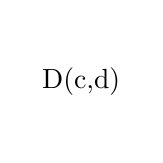
\begin{tikzpicture}[every node/.style={circle, minimum size=8mm}, level/.style={sibling distance=40mm/#1}, level distance=20mm]
        \node {D(c,d)};
    \end{tikzpicture}

    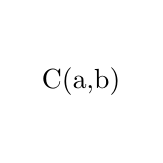
\begin{tikzpicture}[every node/.style={circle, minimum size=8mm}, level/.style={sibling distance=40mm/#1}, level distance=20mm]
        \node {C(a,b)};
    \end{tikzpicture}

    \begin{tikzpicture}[every node/.style={circle, minimum size=8mm}, level/.style={sibling distance=40mm/#1}, level distance=20mm]
        \node {B(a, b, c, d)}
            child {node {C(a,b)}}
            child {node {D(c,d)}};
    \end{tikzpicture}

    \begin{tikzpicture}[every node/.style={circle, minimum size=8mm}, level/.style={sibling distance=40mm/#1}, level distance=25mm]
        \node {A(b, d)}
            child {node {B(a, b, c, d)}
            child {node {C(a,b)}}
            child {node {D(c,d)}}};
            
    \end{tikzpicture}

    The proof tree for $A(b,d)$ already contains proofs for all the other elements of the program so that it would be enough to check this single tree.
\end{example}

We can define an element member function for trees in the usual way:

\begin{lstlisting}
    def elementMember (a: A) (t: tree A): Bool  :=
    match t with
    | tree.node a' l => (a=a') ∨
        List.any l.attach (fun ⟨x, _h⟩ => elementMember a x)
\end{lstlisting}
In order for a tree to be valid all subtrees must be valid. A ground atom $ga$ is exactly then a member of a tree $t$ if there is a subtree of $t$ of which $ga$ is the root, so that if a proof tree is valid all elements are a subset of the semantics.

\begin{lstlisting}
    lemma allTreeElementsOfValidTreeInSemantics 
    (t: proofTree τ)  (P: program τ) (d: database τ) 
    (valid: isValid P d t)(ga:groundAtom τ)(mem: elementMember ga t):
        ga ∈ proofTheoreticSemantics P d :=
\end{lstlisting}

This allows us to establish the alternative property of \texttt{validateTreeList}

\begin{lstlisting}
    lemma validateTreeListUnitIffSubsetSemanticsAndAllElementsHaveValidTrees 
    (P: List (rule τ)) (d: database τ) (l: List (proofTree τ)) 
    (ruleToString: rule τ → String) : validateTreeList P d l  ruleToString = Except.ok () ↔
    {ga: groundAtom τ| ∃ (t: proofTree τ), t ∈ l ∧ elementMember ga t } ⊆ proofTheoreticSemantics P.toFinset d 
    ∧ ∀ (t: proofTree τ), t ∈ l → isValid P.toFinset d t
\end{lstlisting}

Now it is enough to pass just one proof tree from our example to validate the whole input and use in general less trees. 
